Plastic scintillators are easy to machine to any desired shape. The chosen shape for TRITIUM detector is the fiber, specifically, commercial fibers BCF-12 from Saint-Gobain Crystals Inc \cite{DataSheetBCF12Fiber}. This type of fiber was chosen as the result of a comparative study \cite{TFGAlberto} among some of the best-known commercial manufacturers. The BCF-12 fibers consist of scintillating polystyrene core covered by one or two polymethylmethacrylate (PMMA) claddings. % (smaller refractive index than core in order to archieve a critical angle) or a multicladding (second cladding) with even smaller refractive index.

When a particle deposits all or part of its kinetic energy in the scintillating fiber, photons are produced in the fiber core as a result of the fluorescence process. The number of photons produced depends on the production light efficiency of the scintillator (scintillating yield) and its value is around $2.4\%$ for the fibers used (BCF-12), which means that a scintillation yield of about $8000$ photons will be produced per $\MeV$ for a mip. For instance, for tritium electrons of $18.6~\keV$ maximum energy, these fibers release at most 148 photons, probably less as electrons of these energies are not mips. The emission spectrum of the fibers employed in this work, is shown in Figure \ref{fig:EmissionSpectrumFibers}.

\begin{figure}[htbp]
\centering
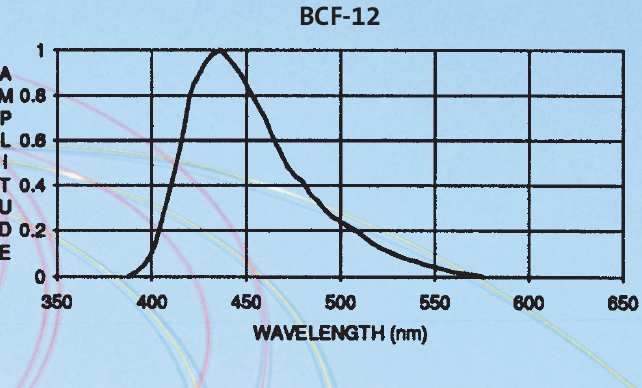
\includegraphics[scale=0.5]{3DesignPrinciples/32Tritium_detector/EmisionBCF12.png}
\caption{Emission spectrum of BCF-12 scintillating fibers of Saint-Gobain\label{fig:EmissionSpectrumFibers}~\cite{DataSheetBCF12Fiber}.}
\end{figure}

The scintillation light is guided to the sensitive part of the photosensor. A single photon produces a signal with some probability, called the quantum efficiency. Fibers (and scintillators in general) use the optical property of Snell's law \cite{Snell} to guide their photons to the desired part (ends of the fibers). The guiding mechanism is determined by the interface between the core and the surrounding material. When a photon hits this interface, it is refracted (and therefore lost) following the Snell equation, \ref{eq:Snell} \cite{Snell}. 
\begin{equation}
n_0~sen(\theta_0) = n_1~sen(\theta_1)
\label{eq:Snell}
\end{equation}
where $\theta_0$ is the incident angle formed by the photon and the surface of in the first environment, with refractive index $n_0$ and $\theta_1$  is the refracted angle formed by the photon and the second environment with refractive index $n_1$. If the surrounding material has a lower refractive index than the core of the fiber, as it is the case with scintillating fibers, there exist a critical angle, $\theta_c$, beyond which photons will be totally reflected ($\theta_1 = 90\degree$) and therefore kept within the fiber as illustrated in Figure \ref{fig:Fiber_physic}.
\begin{equation}
\theta_c = asen\left(\frac{n_1}{n_0} \right)
\label{eq:CriticAngle}
\end{equation}

The trapping efficiency or photon collection efficiency is defined as the efficiency of the scintillator to guide photons. For BCF-12 fibers with optical clad this efficiency is between $3.44\%$ and $7\%$ per meter of fiber (depending on where the event is detected and is minimum near the fiber axis  and maximum near the core-clad interface). Therefore, from the $148$ photons initially created by a tritium decay electron detected with the maximum energy, $18.6~\keV$, and assuming a light yield of $8000$ photons$/\MeV$ according to the manufacturer, only $52$ photons are guided along the $20~\cm$ fiber length of the TRITIUM detector (considering the maximum trapping efficiency ($7\%$) and guessing a linear dependence with the length of the fiber). Thus, the output signal is weak and is in the energy range of the spectrum where electronic noise is already significant. As described in the following chapters, a great effort was made to minimize electronic noise by different techniques. In Figure \ref{fig:Fiber_physic} the light collection in a fiber is illustrated.

\begin{figure}[htbp]
\centering
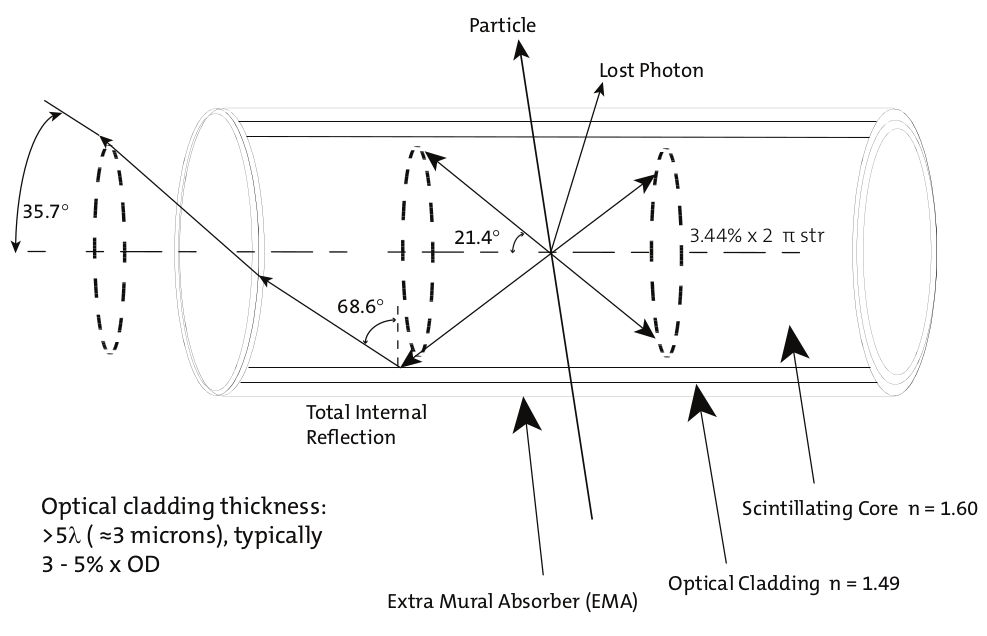
\includegraphics[scale=0.5]{3DesignPrinciples/32Tritium_detector/Fiber_data_sheet.png}
\caption{Photon collection in a single clad fiber\label{fig:Fiber_physic}~\cite{DataSheetBCF12Fiber}.}
\end{figure}

The cladding material has a higher refractive index than air or water. Due to that, this is useful for protecting the core surface from dirt or aggressive external agents that may reduce the light collection but at the cost of increasing the critical angle with its corresponding loss of light. Three different cases are shown in Table \ref{tab:CriticalAngles}, where the cladding effect is illustrated.

\begin{table}[htbp]
\centering{}%
\begin{tabular}{lcc}
\toprule 
Material & Refractive index & critical angle ($\degree$) \tabularnewline
\midrule
\midrule 
Air & 1 & $42.98$ \tabularnewline
Water & 1.33 & $62.47$ \tabularnewline
Cladding of PMMA & 1.49 & $76.26$ \tabularnewline
\bottomrule
\end{tabular}
\caption{Critical angles associated to different interfaces created with polystyrene, $n_0=1.6$, and other materials.}
\label{tab:CriticalAngles}
\end{table}

As can be seen, the trapping efficiency of uncladded fibers BCF-12 surrounded by water or air is larger than for cladded fibers. However, in the practice, it is difficult to achieve a perfect air-core or water-core interface, and this affects light collection. As commercial claddings are thicker ($30~\micro \meter$) than the mean free path of tritium decay electrons in water (around $5~\micro\meter$), cladded fibers are not an option for the TRITIUM detector. Hence, special attention is needed for achieving a good enough water-core interface. To achieve this goal a special method was developed in the ICMOL laboratory for preparing fibers for tritium detection, detailed and tested in section \ref{subsec:CleaningProcess}. The relevant parameters of scintillating fibers used for TRITIUM detector are given in Table \ref{tab:ParametersFibersBCF12}.

\begin{table}[htbp]
\centering{}%
\begin{tabular}{lc}
\toprule 
Property & Value \tabularnewline
\midrule
\midrule 
Core material & Polystyrene \tabularnewline
Core refractive index & 1.60 \tabularnewline
Density ($\gram/\cm^3$) & 1.05 \tabularnewline
Cladding material & Acrylic (PMMA) \tabularnewline
Cladding refractive index & 1.49 \tabularnewline
Cladding thickness & $3\%$ \tabularnewline
Numerical aperture & 0.58 \tabularnewline
Trapping efficiency & 3.44\% minimum \tabularnewline
No. of H atoms per cc (core) & $4.82 \cdot{} 10^{22}$ \tabularnewline
No. of C atoms per cc (core) & $4.85 \cdot{} 10^{22}$ \tabularnewline
No. of electrons per cc (core) & $3.4 \cdot{} 10^{23}$ \tabularnewline
Radiation lenght (cm) & 42 \tabularnewline
Emission peak (nm) & 435 (Blue) \tabularnewline
Decay Time, (ns) & 3.2 \tabularnewline
1/e Length (m) & 2.7 \tabularnewline
Scintillator yield (\#$\gamma$/MeV) & $\sim 8000$ \tabularnewline
Operating Temperature & $-20\degree C$ to $50\degree C$ \tabularnewline
\bottomrule
\end{tabular}
\caption{Properties of BCF-12 fibers from Saint-Gobain Inc. \cite{DataSheetBCF12Fiber}.}
\label{tab:ParametersFibersBCF12}
\end{table}